\documentclass{article}
\usepackage{tikz}
\usetikzlibrary{positioning}

\begin{document}

\begin{figure}[h]
    \centering
    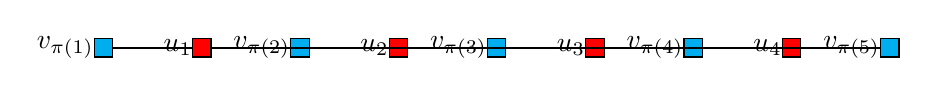
\begin{tikzpicture}[node distance=1cm, auto]
        % Define nodes
        \node[draw, fill=cyan] (v1) {};
        \node[draw, fill=red] (u1) [right=of v1] {};
        \node[draw, fill=cyan] (v2) [right=of u1] {};
        \node[draw, fill=red] (u2) [right=of v2] {};
        \node[draw, fill=cyan] (v3) [right=of u2] {};
        \node[draw, fill=red] (u3) [right=of v3] {};
        \node[draw, fill=cyan] (v4) [right=of u3] {};
        \node[draw, fill=red] (u4) [right=of v4] {};
        \node[draw, fill=cyan] (v5) [right=of u4] {};

        % Draw edges
        \draw[thick, black] (v1) -- (u1);
        \draw[thick, black] (v2) -- (u2);
        \draw[thick, black] (v3) -- (u3);
        \draw[thick, black] (v4) -- (u4);

        % Draw arcs
        \draw[thick, black] (u1) to[out=0,in=180] (v5);

        % Add labels
        \node at (v1) [left] {$v_{\pi(1)}$};
        \node at (u1) [left] {$u_1$};
        \node at (v2) [left] {$v_{\pi(2)}$};
        \node at (u2) [left] {$u_2$};
        \node at (v3) [left] {$v_{\pi(3)}$};
        \node at (u3) [left] {$u_3$};
        \node at (v4) [left] {$v_{\pi(4)}$};
        \node at (u4) [left] {$u_4$};
        \node at (v5) [left] {$v_{\pi(5)}$};
    \end{tikzpicture}
\end{figure}

\end{document}